% thios section describes the computational image complexity analysis

a Python script that processes images to produce complexity scores.
This section of your methodology will delve into the technical aspects of the complexity analysis process using Python scripting and image data.

The theory framework section explored in detail the evolution of architecture, and it was concluded that there is an apparent cycle in the history of architecture that fluctuates between complex and simple styles.
The recent development in technology in addition with the most recent architectural styles suggests that the contemporary era will tilt towards a more complex approach as a response to the previous Modernist movement based on minimalism and simplicity.

To prove this hypothesis a computational complexity analysis system was conceptualized, based on the idea of quantifying the level of complexity of a building as objectively as possible to eliminate possible bias from the theory analysis. indicates the advent of a new style that tilts towards complexity.

%% Figure Methodology flowchart
    \begin{figure}[!htb]
      \centering
      % trim=left 190 down 250 right 150 top5
      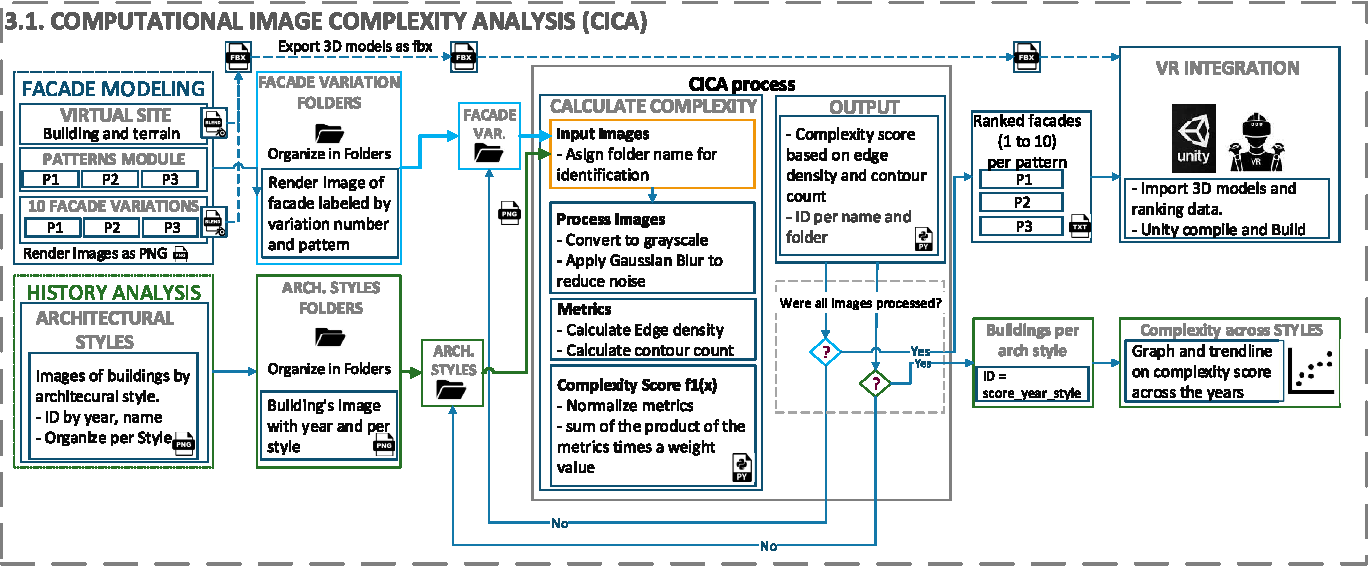
\includegraphics[width= \linewidth, trim=0 0 0 0, clip]{Images/ImageComplexityAnalysisFlowchart}
      \caption{Flowchart illustrating the applications of Computational Image Complexity Analysis, including its role in analyzing complexity scores for historical architectural styles and ranking modeled facades for the VR Building Complexity System.}
      \label{fig:ImageComplexityAnalysisFlowchart}
    \end{figure}